\documentclass[12pt]{article}%
\usepackage{amsmath}
\usepackage{amssymb}
\usepackage{graphicx}


\begin{document}

\newcommand\scalemath[2]{\scalebox{#1}{\mbox{\ensuremath{\displaystyle #2}}}}
\title{Machine Learning \protect\\ Assignment 2 \protect\\ CLO3 Exercise 18} 
\author{Ida Bagus Dwi Satria Kusuma \protect\\ 1301140297}
\date{\today}
\maketitle

\begin{enumerate}
	\item In this exercise we will implement SVM for non-linearly separable data.
	\begin{enumerate}
		\item \textbf{(5 points)} Load the selected data set. Visualize all data points using scatter plot. Use different color or symbol for each class. Use attribute 1 as x -axis, attribute 2 as y -axis.

		\par \textbf{Jawab:} Visualisasi data menggunakan \textit{scatter plot}, di mana simbol '+' biru adalah data dengan kelas '1' dan simbol 'o' merah adalah data dengan kelas '-1'.
		\par 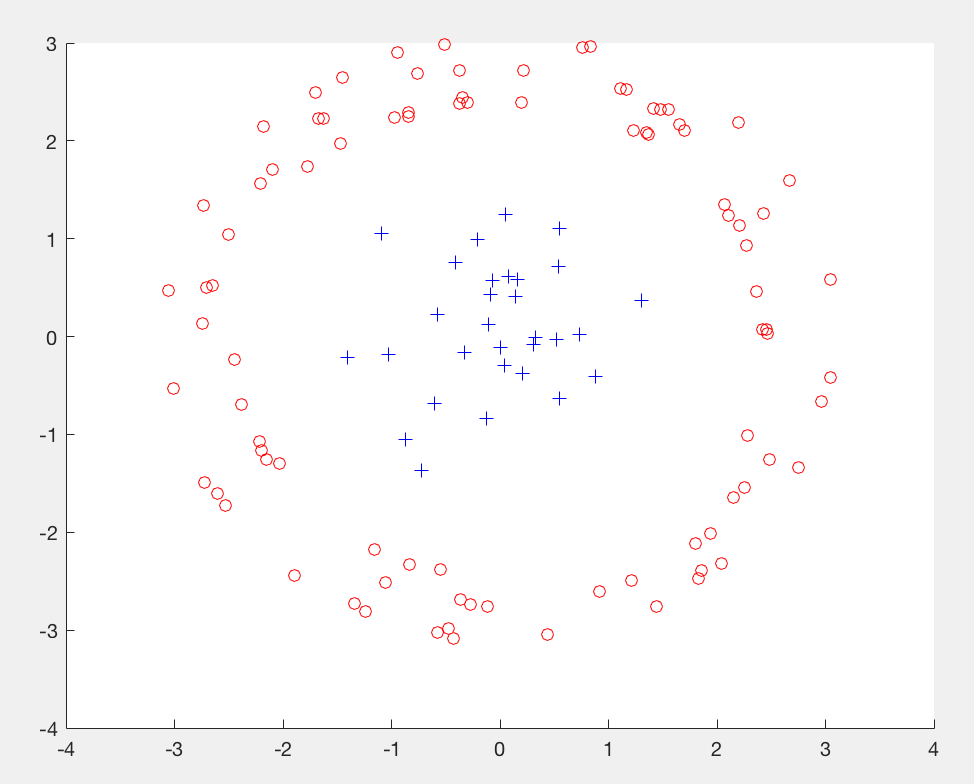
\includegraphics[width=10cm]{ass2clo3no18_1} 

		\item (10 points) Create a function that implements polynomial kernel. Inputs for the function are attributes ($x_1$ and $x_2$). The function transforms data from original feature space into new feature space. Here we transform data from 2 dimensional space into 3 dimensional space, $\Phi:\mathbb{R}^2 \rightarrow \mathbb{R}^3$ ,that is transforming $\textbf{x}=(x_1,x_2)$into $\textbf{z}=(z_1,z_2,z_3)=(x_1,x_2,x^2_1+x^2_1)$.

		\par
		\par 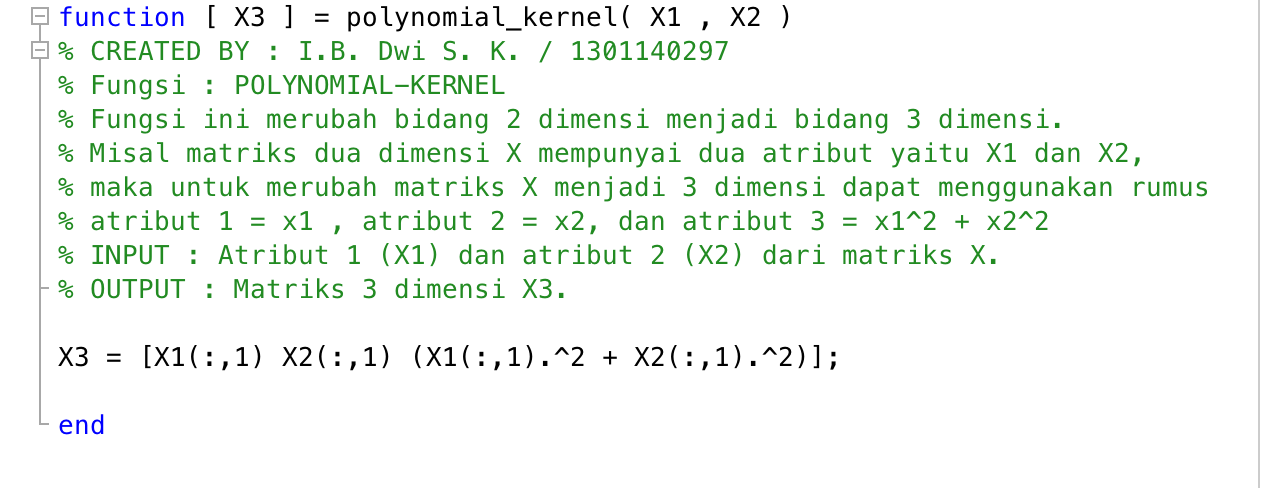
\includegraphics[width=10cm]{ass2clo3no18_2} 

		\item (5 points) In a new feature space, $\mathbb{R}^3$, visualize all data points using scatter plot in one color, and use different symbols for each class, for example class ’-1’ uses symbol ’o’ while class ’1’ uses symbol ’+’).

		\par 
		\par 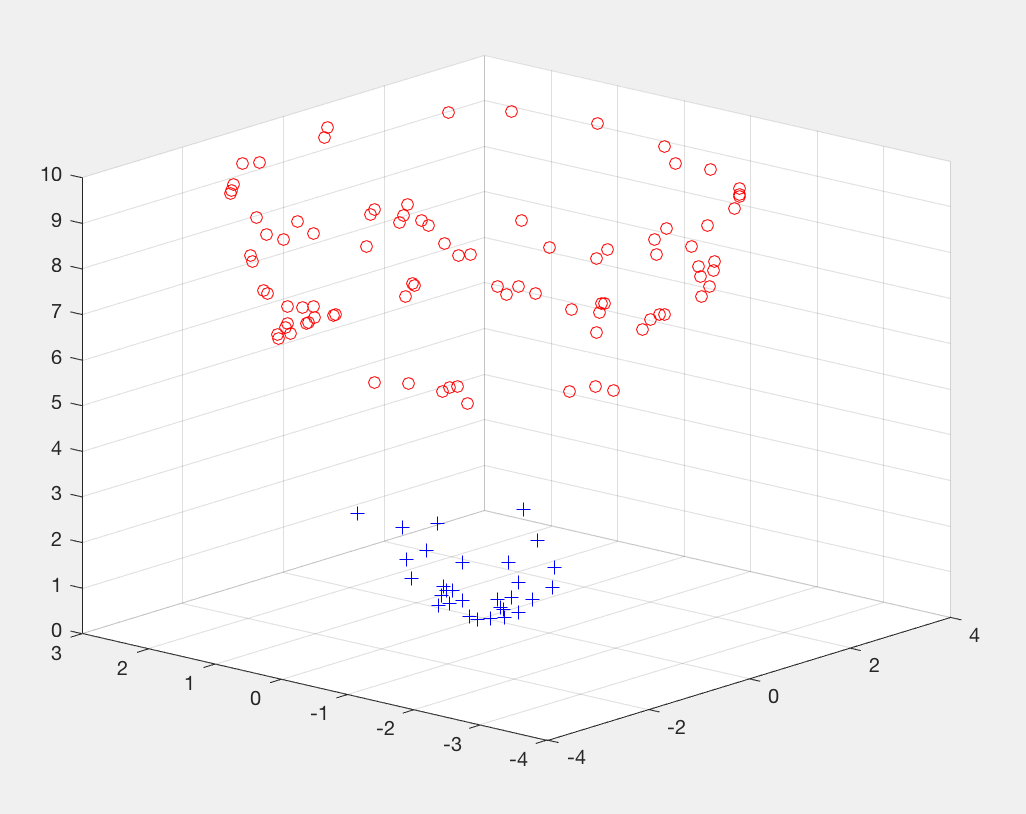
\includegraphics[width=10cm]{ass2clo3no18_3} 
		\par Kelas '-1' direpresentasikan dengan simbol 'o' merah, dan kelas '1' direpresentasikan dengan simbol '+' biru.


		\item (20 points) Using quadratic programming library, find the vector $\textbf{w}$ and $b$ that construct the hyperplane for classifying the data set in $\mathbb{R}^3$,

		\par \textbf{Jawab:} Untuk mencari nilai $\textbf{w}$ dan $b$, kita dapat menggunakan \textit{quadratic programming}, namun sebelumnya, kita harus mentransformasikan data dari $\mathbb{R}^2$ menjadi $\mathbb{R}^3$. Untuk detail lebih jelasnya, menggunakan code berikut :

		\par 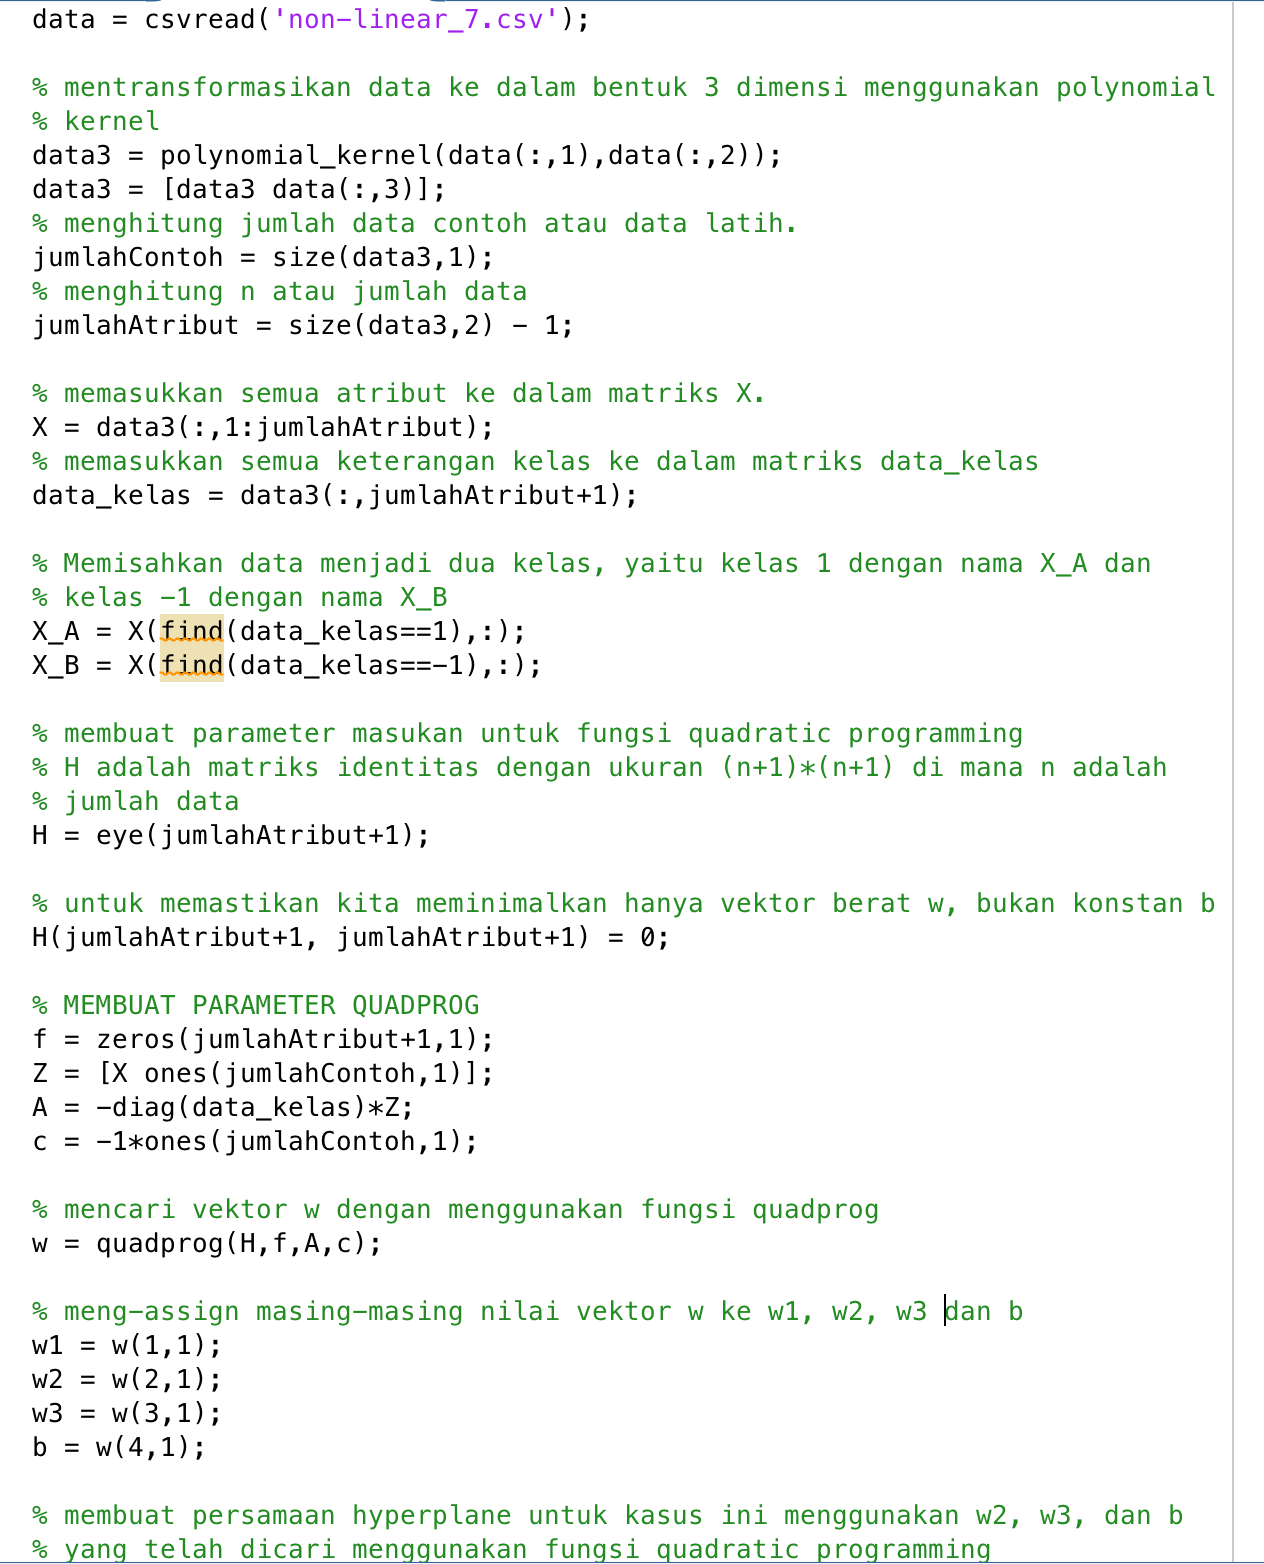
\includegraphics[width=10cm]{ass2clo3no18_4}
		\par 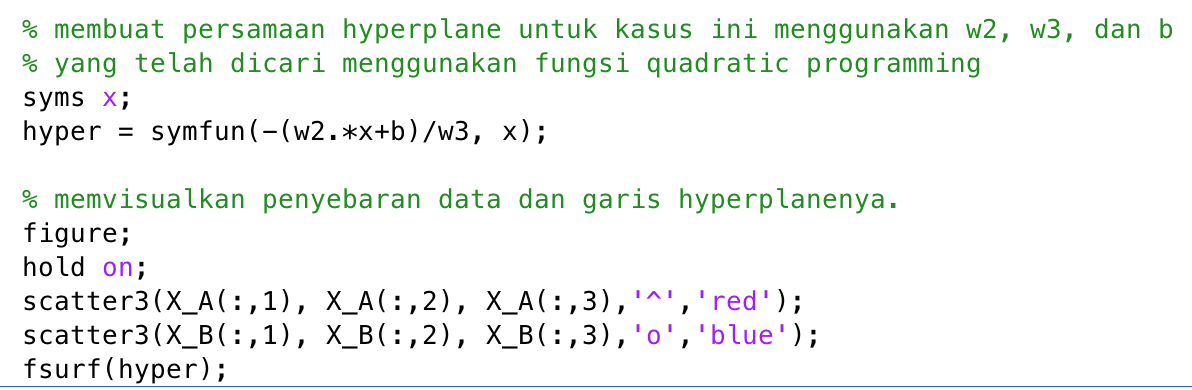
\includegraphics[width=10cm]{ass2clo3no18_5}  

		\par
		\par Setelah itu, kita mendapatkan masing-masing nilai $w_1, w_2, w_3$ dan $b$
		\par 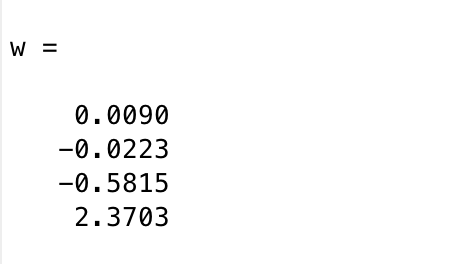
\includegraphics[width=10cm]{ass2clo3no18_6}

		\par $w_1 = 0.0090$, $w_2 = -0.0223$, $w_3 = 0.5815$ dan $b = 2.3703$. Persamaan hyperplanenya adalah 

		\begin{align*}
		 	hyperplane & = \frac{-(w_2 \times x + b)}{w_3} \\
		 	& = \frac{-(-0.0223 \times x + 2.3703)}{-0.5814}
		\end{align*}

		\item (5 points) Now visualize the hyperplane on the scatter plot that is created on 18(d). Oneof online articles that you could learn on how to visualize the hyperplane for this exercise using Octave/Matlab is here or go to next url: https://se.mathworks.com/matlabcentral/ answers/104248-implementation-support-vector-machine-nonlinear-case-with-quadprog- function-in-matlab. For python, Java, C++ and so on, you could search it on internet.

		\par \textbf{Jawab:} Dengan menggunakan persamaan \textit{hyperplane} pada nomor 18(d), visualisasi dari \textit{hyperplane}-nya :

		\par 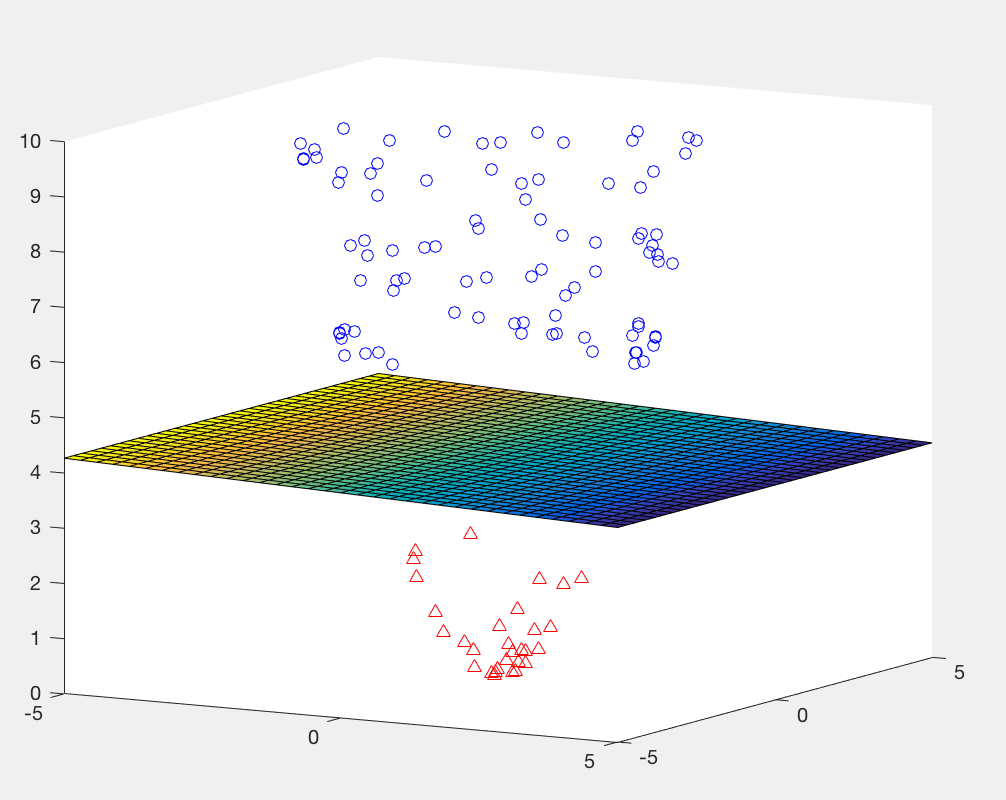
\includegraphics[width=10cm]{ass2clo3no18_7}	
		\par 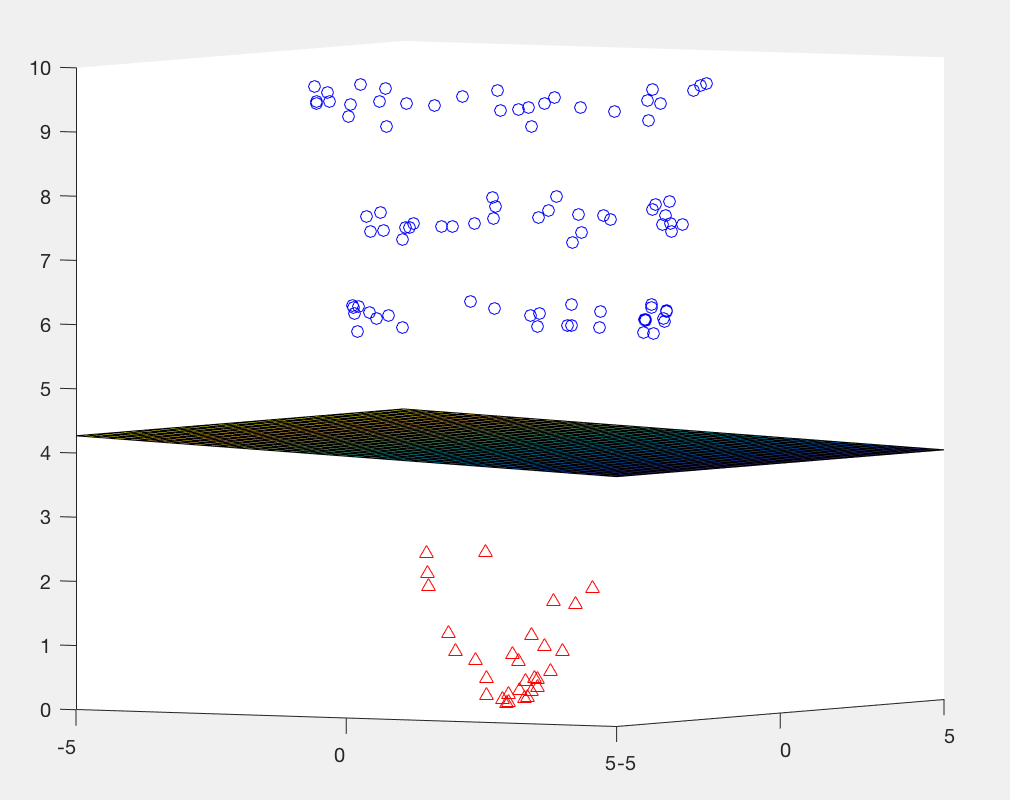
\includegraphics[width=10cm]{ass2clo3no18_8}
	\end{enumerate}
	


\end{enumerate}

\par \textbf{Referensi}
\par [1] https://id.wikipedia.org/wiki/Regresi\_Linier
\par [2] Introduction to Data Mining - Panning Tan, M. Steinbach
\par [3] https://en.wikipedia.org/wiki/Nonlinear\_regression
\par [4] Regression book
\par [5] Regression slide
\par [6] http://www.nickgillian.com/wiki/pmwiki.php/GRT/MLP
\par [7] Machine Learning - Tom Mitchell
\par [8] https://medium.com/towards-data-science/activation-functions-and-its-types-which-is-better-a9a5310cc8f
\par [9] Slide ANN-MLP Machine Learning
\par [10] https://www.mathworks.com/help/optim/ug/quadprog.html#inputarg\_f
\par [11] http://www.robots.ox.ac.uk/~az/lectures/ml/ matlab2.pdf
\par [12] https://se.mathworks.com/matlabcentral/ answers/104248-implementation-support-vector-machine-nonlinear-case-with-quadprog- function-in-matlab


\end{document}

